\documentclass[12pt,letterpaper]{article}
\usepackage[utf8]{inputenc}
\usepackage[spanish]{babel}
\usepackage{graphicx}
\usepackage[left=2cm,right=2cm,top=2cm,bottom=2cm]{geometry}
\usepackage{graphicx} % figuras
% \usepackage{subfigure} % subfiguras
\usepackage{float} % para usar [H]
\usepackage{amsmath}
%\usepackage{txfonts}
\usepackage{stackrel} 
\usepackage{multirow}
\usepackage{enumerate} % enumerados
\renewcommand{\labelitemi}{$-$}
\renewcommand{\labelitemii}{$\cdot$}
% \author{}
% \title{Caratula}
\begin{document}

% Fancy Header and Footer
% \usepackage{fancyhdr}
% \pagestyle{fancy}
% \cfoot{}
% \rfoot{\thepage}
%

% \usepackage[hidelinks]{hyperref} % CREA HYPERVINCULOS EN INDICE

% \author{}
\title{Caratula}

\begin{titlepage}
\begin{center}
\large{UNERSIDAD PRIVADA DE TACNA}\\
\vspace*{-0.025in}
\begin{figure}[htb]
\begin{center}

\includegraphics[width=8cm]{./Imagenes/logo}
\end{center}
\end{figure}
\vspace*{0.15in}
INGENIERIA DE SISTEMAS  \\

\vspace*{0.5in}
\begin{large}
TITULO:\\
\end{large}

\vspace*{0.1in}
\begin{Large}
\textbf{ Guia de Instalacion y Configuracion de Base de Datos} \\
\end{Large}

\vspace*{0.3in}
\begin{Large}
\textbf{CURSO:} \\
\end{Large}

\vspace*{0.1in}
\begin{large}
BASE DE DATOS II\\
\end{large}

\vspace*{0.3in}
\begin{Large}
\textbf{DOCENTE(ING):} \\
\end{Large}

\vspace*{0.1in}
\begin{large}
 Patrick Cuadros Quiroga\\
\end{large}

\vspace*{0.2in}
\vspace*{0.1in}
\begin{large}
Integrante: \\
\begin{flushleft}
Balaguer Valles Angela Lessly		\hfill	(2016054494) \\
Huallpa Castro Leydi Katherine 		\hfill	(2015053230) \\
Mamani Ayala Brandon 	           	\hfill	(2015052715) \\
Pilco Quispe Mireya Flavia      		\hfill	(2015053234) \\
Quispe Mamani Angelo 	  		\hfill	(2015052826) \\
Vizcarra Llanque Jhordy 			\hfill	(2015052719) \\
\end{flushleft}
\end{large}
\end{center}

\end{titlepage}


\tableofcontents % INDICE
\thispagestyle{empty} % INDICE SIN NUMERO
\newpage
\setcounter{page}{1} % REINICIAR CONTADOR DE PAGINAS DESPUES DEL INDICE


\section{Parte 01 - Definiciones} 

\begin{enumerate}[1.]
	\item OBJETIVOS
	\\\\- Brindar al estudiante los conocimientos necesarios para realizar la Instalación de un servidor de Base de Datos Oracle sobre el sistema operativo Windows Server 2012 R2.
	\\- Otorgar al estudiante los conocimientos necesarios para realizar la instalación de este servidor dentro de un ambiente virtualizado.\\
	\item REQUERIMIENTOS
	\\-Conocimientos
	\subitem Para el desarrollo de esta práctica se requerirá de los siguientes conocimientos básicos:

	\item CONSIDERACIONES INICIALES
	\subitem Conocimientos b\'asicos como usuario de Windows Server 2012 R2
	\subitem Conocimientos b\'asicos sobre software virtualizador VMware Workstation
	\subitem Conocimientos b\'asicos en configuración de Oracle Database 12

\end{enumerate} 

\section{Parte 02 – Instalacion de VMWare} 

\begin{enumerate}[1.]
	\item Paso 01 : ejecutar el instalador de VMware y seleccionar en todas las ventanas el boton next
	
	\begin{center}
	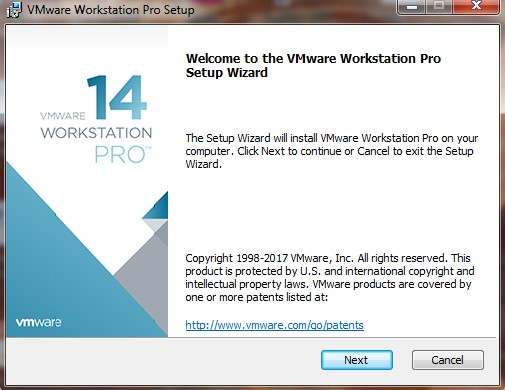
\includegraphics[width=10cm]{./Imagenes/WM01} 
	\end{center}

	\item Paso 02 :

	\begin{center}
	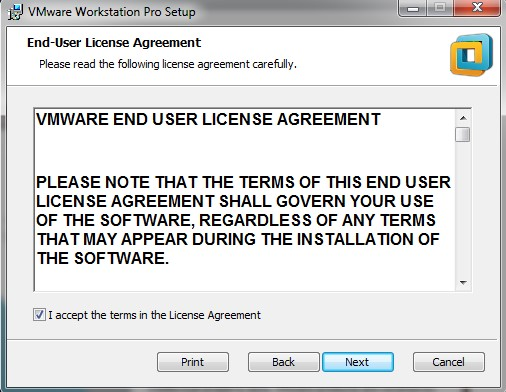
\includegraphics[width=10cm]{./Imagenes/WM02} 
	\end{center}

	\hfill \break
	\hfill \break
	\hfill \break
	\hfill \break
	\hfill \break
	\hfill \break
	\item Paso 03 :

	\begin{center}
	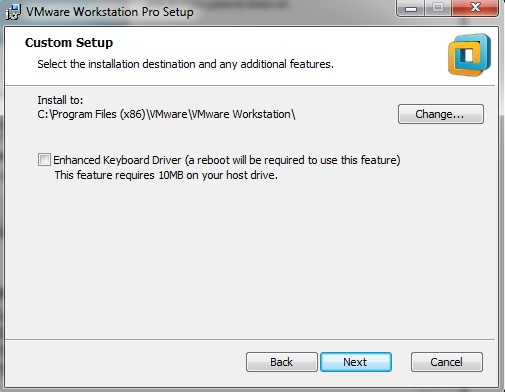
\includegraphics[width=10cm]{./Imagenes/WM03} 
	\end{center}

	\item Paso 04 :

	\begin{center}
	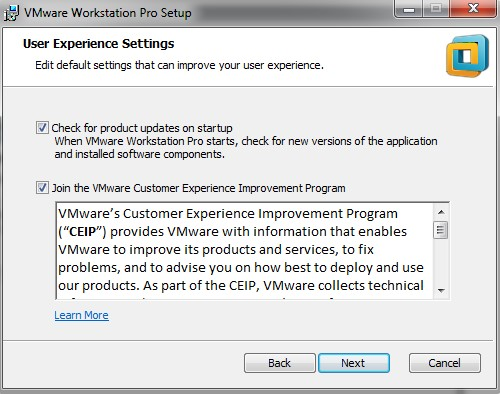
\includegraphics[width=10cm]{./Imagenes/WM04} 
	\end{center}

	\hfill \break
	\hfill \break
	\hfill \break
	\hfill \break
	\hfill \break
	\hfill \break
	\hfill \break
	\hfill \break
	\item Paso 05 : ahora ya instalamos el programa

	\begin{center}
	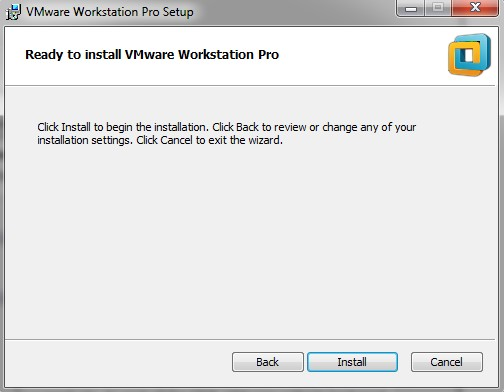
\includegraphics[width=10cm]{./Imagenes/WM05} 
	\end{center}

	\item Paso 06 :

	\begin{center}
	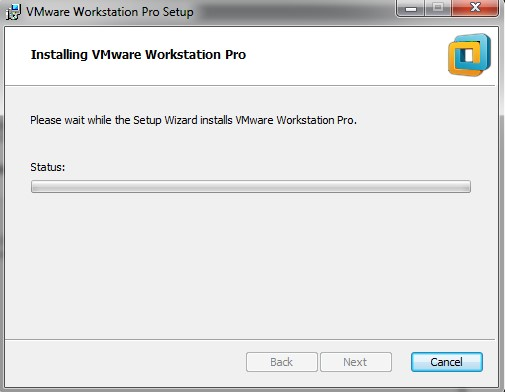
\includegraphics[width=10cm]{./Imagenes/WM06} 
	\end{center}

	\hfill \break
	\hfill \break
	\hfill \break
	\hfill \break
	\hfill \break
	\hfill \break
	\hfill \break
	\hfill \break
	\item Paso 07 :

	\begin{center}
	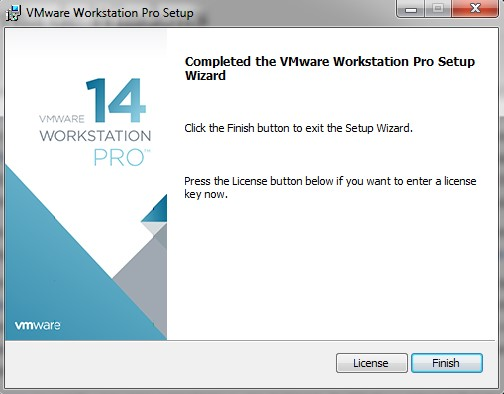
\includegraphics[width=10cm]{./Imagenes/WM07} 
	\end{center}

	\item Paso 08 : Ingresamos la clave del producto

	\begin{center}
	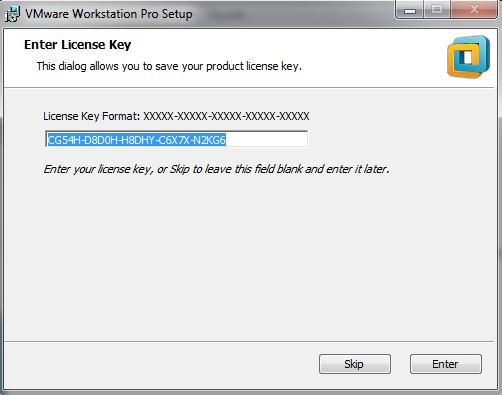
\includegraphics[width=10cm]{./Imagenes/WM08} 
	\end{center}

	\hfill \break
	\hfill \break
	\hfill \break
	\hfill \break
	\hfill \break
	\hfill \break
	\hfill \break
	\hfill \break

\end{enumerate} 

\section{Parte 03 – Instalacion de Windows Server} 


\section{Parte 04 – Instalacion de Oracle Data 12C} 
\begin{enumerate}[1.]
	      
	\item Ingresamos nuevamente a Administraci\'on de equipos y seleccionamos  la opci\'on de usuarios y grupos locales.\\
	\begin{center}
	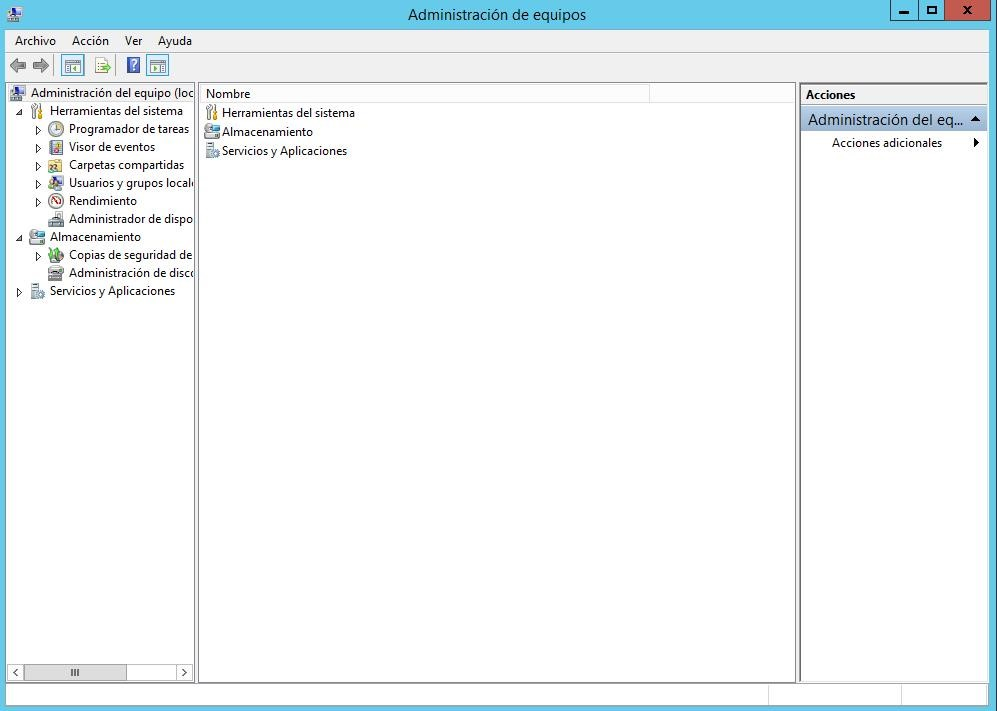
\includegraphics[width=10cm]{./Imagenes/jhordy1} 
	\end{center}
	\hfill \break	
	\hfill \break
	\hfill \break
	\hfill \break
	\begin{center}
	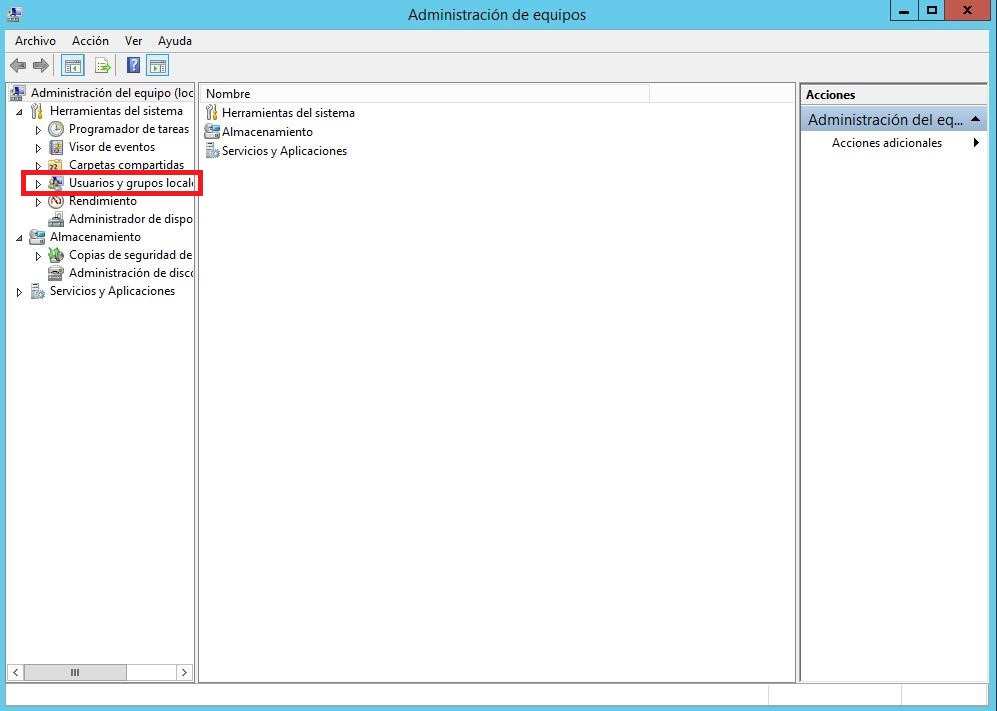
\includegraphics[width=10cm]{./Imagenes/jhordy11} 
	\end{center}
	\hfill \break
	\hfill \break
	\hfill \break
	\hfill \break
	\item Ingresamos a la carpeta de Usuarios y nos vamos a la opci\'on de equipos ORACLE.\\
	\begin{center}
	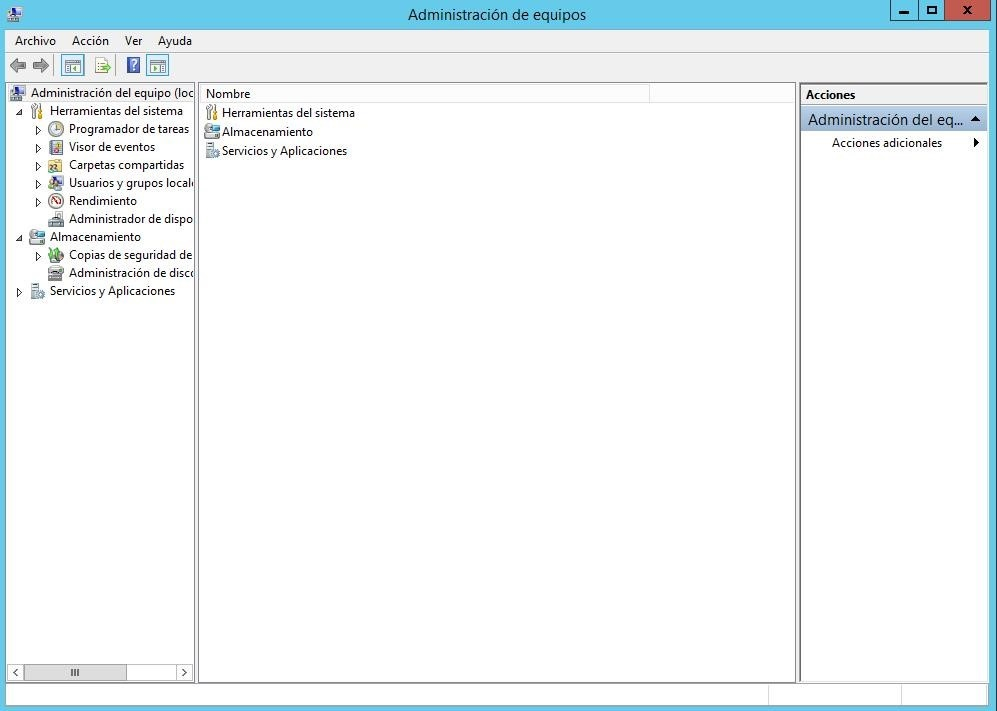
\includegraphics[width=10cm]{./Imagenes/jhordy2} 
	\end{center}
	\hfill \break
	\hfill \break
	\hfill \break
	\hfill \break
	\item Una vez realizado eso reiniciamos el servidor y al usuario ORACLE.\\
	\begin{center}
	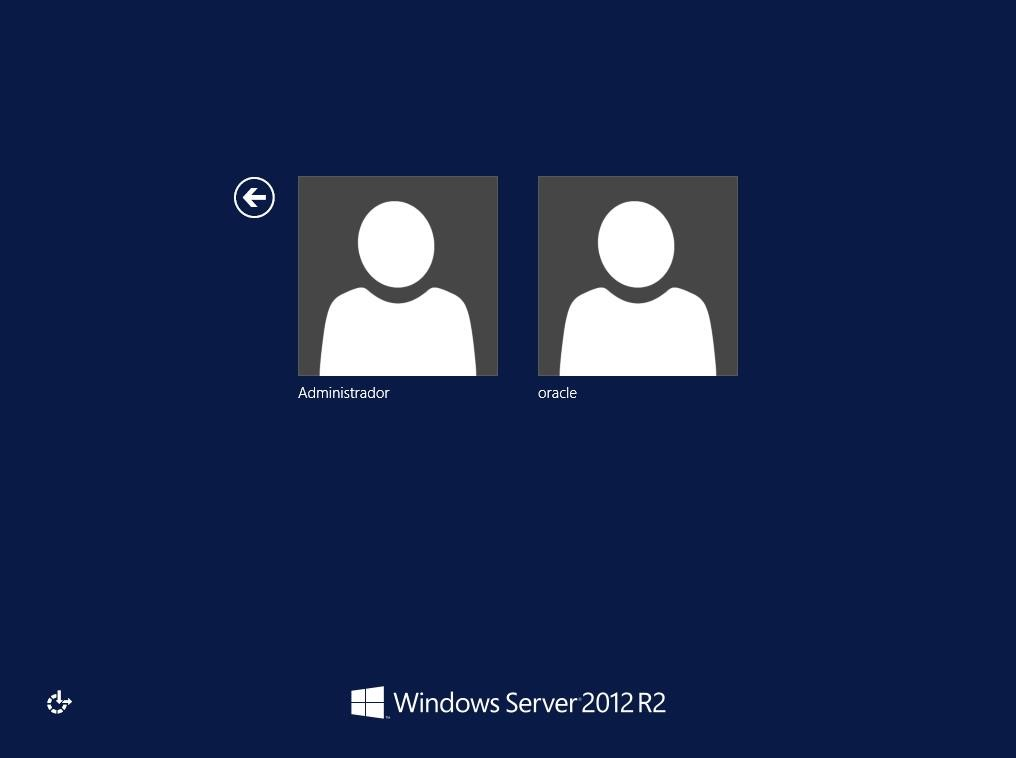
\includegraphics[width=10cm]{./Imagenes/jhordy3} 
	\end{center}
	\hfill \break
	\hfill \break
	\hfill \break
	\hfill \break
	\item Colocamos la clave de administrador que es  "UPT2018".\\
	\begin{center}
	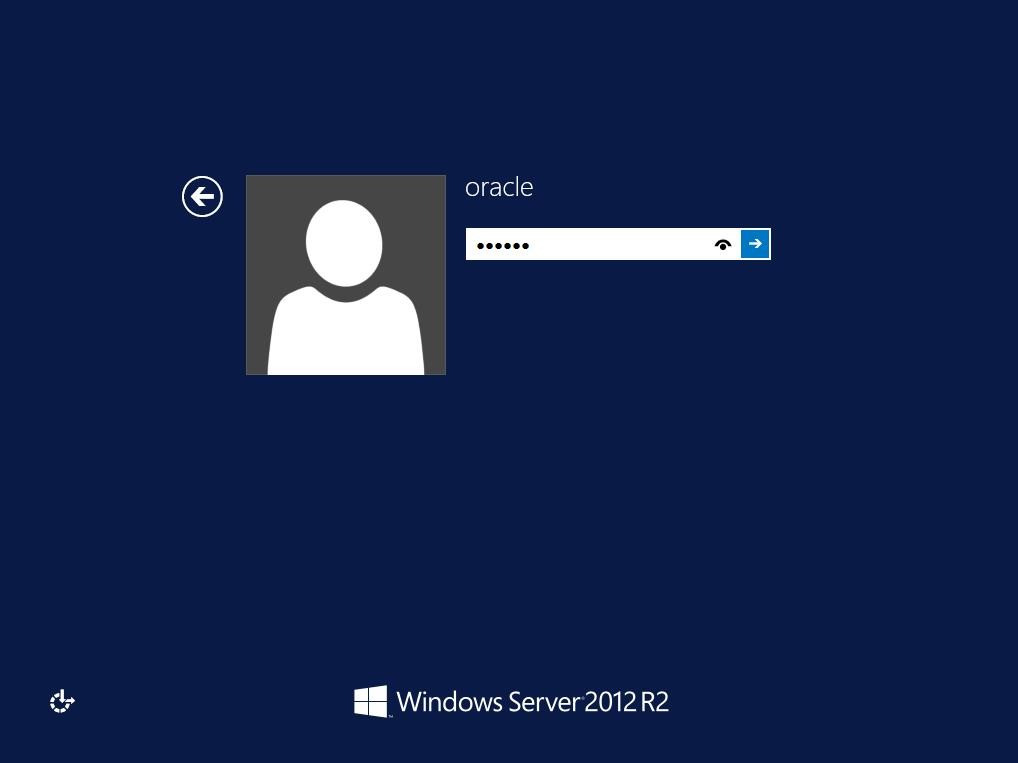
\includegraphics[width=10cm]{./Imagenes/jhordy4} 
	\end{center}
	\hfill \break
	\hfill \break
	\hfill \break
	\hfill \break
	\item Empezaremos la instalaci\'on de la base de datos ORACLE seleccionando el archivo ejecutable "setup" a setup.\\
	\begin{center}
	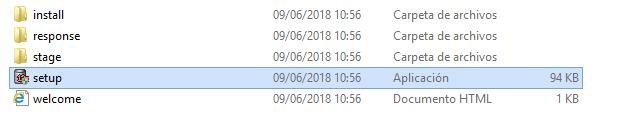
\includegraphics[width=10cm]{./Imagenes/jhordy5} 
	\end{center}
	\hfill \break
	\hfill \break
	\hfill \break
	\hfill \break
	\hfill \break
	\item Instalamos como el usuario administrador, colocando la clave de usuario.\\
	\begin{center}
	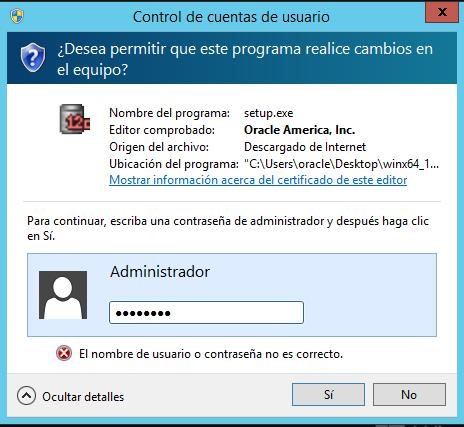
\includegraphics[width=10cm]{./Imagenes/jhordy6} 
	\end{center}
	\hfill \break
	\hfill \break
	\hfill \break
	\hfill \break
	\item Procede autom\'aticamente la instalaci\'on del ORACLE\\
	\begin{center}
	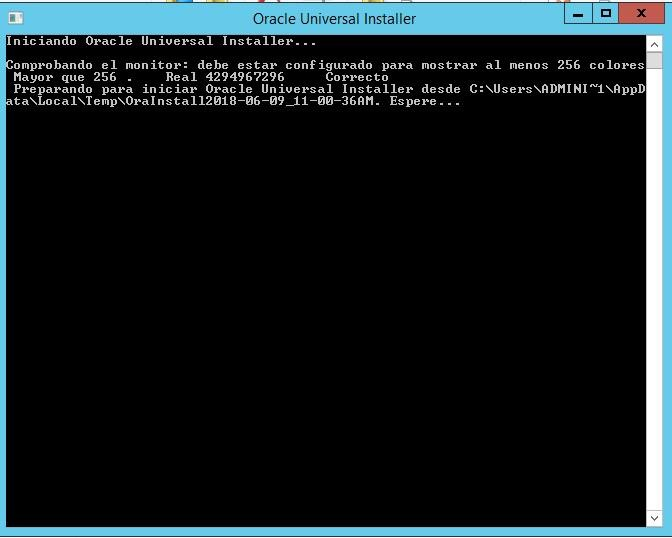
\includegraphics[width=10cm]{./Imagenes/jhordy7} 
	\end{center}
	\hfill \break
	\hfill \break
	\hfill \break
	\hfill \break
	\hfill \break
	\hfill \break
	\hfill \break
	\hfill \break
	\hfill \break
	\item Nos aparece la pantalla de configuraci\'on.\\
	\begin{center}
	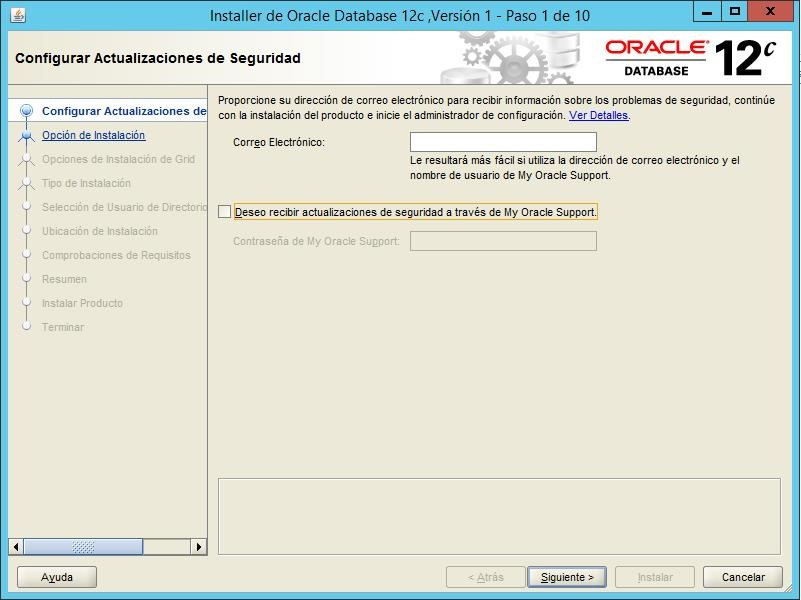
\includegraphics[width=10cm]{./Imagenes/jhordy8} 
	\end{center}
	
\end{enumerate} 

\include{Secciones/Actividad05}



\end{document}
